%% SLIDE 1
% Introduzione alla tecnologia ARTVA
\newslide{ARTVA Beacons Overview}{
\begin{block}{}
\centering
\begin{tikzpicture}[node distance=5mm,>=latex']
	%%
	% Immagine di un artva digitale
 	\begin{scope}[local bounding box=artva]
 		\node [rectangle, inner sep=4pt] (digitalartva) {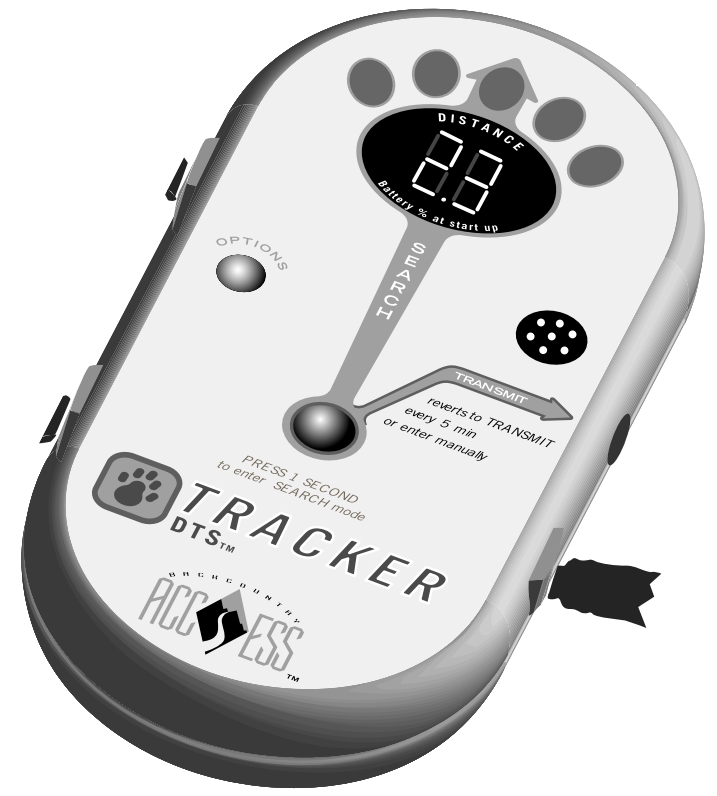
\includegraphics[width=4cm]{img/digital_baecon.png}}; % i know i know... mistype...
 	\end{scope}

 	%% 
 	% Grafico di funzionamento di un artva digitale
 	%\begin{scope}[local bounding box=receiver, auto,node distance=1cm,>=latex', shift={($(artva.north east)+(5cm,0)$)},inner sep=2pt]	
 	\node [rectangle, inner sep=4pt,name=receiver, at=(artva.east), anchor=west, xshift=3cm] { 
 		\begin{tikzpicture}[auto,node distance=1cm,>=latex']
	 		\node[regular polygon, regular polygon sides=3, regular polygon rotate=180, draw, minimum height=1cm] (ant) {};
			\draw (ant.north) -- (ant.south);
			
			\node[below of=ant] (input) {};
			\begin{scope}[node distance=4mm and 6mm]
				\node[rectangle, draw, right=of input, minimum width=2.3cm, text width=2cm, align=center] (b1) {\scriptsize{Triple Antennas}};
				\node[rectangle, draw, right=of b1, minimum width=2.3cm, text width=2cm, align=center] (b2) {\scriptsize{Frequency shift \\ Anti--alias filter}};
				\node[rectangle, draw, below=of b2, minimum width=2.3cm, text width=2cm, align=center] (b3) {\scriptsize{A--D \\ Conversion}};
				\node[rectangle, draw, below=of b3, minimum width=2.3cm, text width=2cm, align=center] (b4) {\scriptsize{Digital Filter}};
				\node[rectangle, draw, left=of b4, minimum width=2.3cm, text width=2cm, align=center] (b5) {\scriptsize{Signal \\ Detection}};
				\node[rectangle, draw, left=of b5, minimum width=2.3cm, text width=2cm, align=center] (b6) {\scriptsize{H--field \\ Estimation}};
			\end{scope}

			\draw[->] (ant.south) |- (b1) {};
			\draw[->] (b1) -- (b2) {};
			\draw[->] (b2) -- (b3) {};
			\draw[->] (b3) -- (b4) {};
			\draw[->] (b4) -- (b5) {};
			\draw[->] (b5) -- (b6) {};
			\node [at=(b3.0), anchor=(180), shift=(0:3mm)] (n1) {};
			\node [at=(b3.0), anchor=(180), shift=(180:88mm)] (n2) {};
			\draw [dashed] (n2) -- (b3) {};
			\draw [dashed] (n1) -- (b3) {};

			\node [at=(n2.0), anchor=(180), shift=(25:7mm)] (n1) {Analog};
			\node [at=(n2.0), anchor=(180), shift=(-25:7mm)] (n1) {Digital};
		\end{tikzpicture}
	};	

	%%
	% Rappresentazione di un segnale ARTVA 
	\node  [rectangle, inner sep=4pt,name=transmission, at=(receiver.south east), anchor=north east, yshift=-5mm] {
		\begin{tikzpicture}
			\node [text width=5cm] (listitem) {
				{\small
				\begin{itemize}
				\item A1A Signal:
					\begin{itemize}
					\item amplitude modulated digital signal
					\item one carrier frequency: \num{457}\si{\kilo\hertz}
					\item frequency error $\pm$\num{80}\si{\hertz}
					\end{itemize}
				\item H--field peak at \num{10}\si{\meter}
					\begin{itemize}
					\item $\geq 0.5$ \si{\micro\ampere\per\meter}
					\item $\leq 2.23$ \si{\micro\ampere\per\meter}
					\end{itemize}
				\end{itemize}
				}
			};
			\node [right=of listitem] {
				\begin{tikzpicture}[>=latex]
					\draw [->] (0,0) -- node[below,pos=0.5]{\scriptsize{Time}} (3.5,0) node[anchor=west]{\scriptsize{$x$}};
					\draw [->] (0,0) -- node[above,pos=0.75,rotate=90]{\scriptsize{Intelligence}} node[left,pos=0.1,yshift=-8,xshift=-1.5]{0} node[left,pos=0.4,yshift=3,xshift=-1.5]{1} (0,3.5) node[anchor=south]{\scriptsize{$y$}};
					\draw [line width=1.25] (0.1,0.1) -- ++(0.4,0) -- ++(0,1.5) -- ++(1,0) -- ++(0,-1.5) -- ++(1.3,0) -- ++(0,1.5) -- ++(0.5,0);

					\coordinate (start) at (0.5,1.7);
					\coordinate (mid) at (1.5,1.7);
					\coordinate (stop) at (2.8,1.7);
					\coordinate (pA) at (0.5,1.7+1.3);
					\coordinate (pB) at (2.8,1.7+1.3);
					\coordinate (pC) at (0.5,1.7+0.5);
					\coordinate (pD) at (1.5,1.7+0.5);
					\coordinate (pE) at (2.8,1.7+0.5);

					\draw (start) -- (pA) -- ++(0,0.1);
					\draw (stop) -- (pB) -- ++(0,0.1);
					\draw (mid) -- (pD) -- ++(0,0.1);

					\draw [<->] (pC) -- (pD) node[above, pos=0.5]{\scriptsize{$\geq70ms$}};	
					\draw [<->] (pD) -- (pE) node[above, pos=0.5]{\scriptsize{$\geq400ms$}};	
					\draw [<->] (pA) -- (pB) node[above, pos=0.5]{\scriptsize{$1000\pm300ms$}};	
				\end{tikzpicture}
			};
		\end{tikzpicture}
	};

	\draw [line width=1.5,->] (digitalartva.east) -- node[above] {RX MODE} (receiver.west);
	\draw [line width=1.5,->] (digitalartva.south) |- node[below, pos=0.7] {TX MODE} (transmission.west);
\end{tikzpicture}
\end{block}
}